\documentclass[10pt,journal,compsoc]{IEEEtran}
\usepackage{cite}
\usepackage{amsmath,amssymb,amsfonts}
\usepackage{algorithmic}
\usepackage{graphicx}
\usepackage{textcomp}
\usepackage{xcolor}
\usepackage{booktabs}
\usepackage{hyperref}

\def\BibTeX{{\rm B\kern-.05em{\sc i\kern-.025em b}\kern-.08em
    T\kern-.1667em\lower.7ex\hbox{E}\kern-.125emX}}

\begin{document}

\title{Evaluating Subspace Orthogonality and Sparse Low-Rank Adaptation under Model-Directed Curricula in Autonomous Self-Editing Language Models}

\author{Honours Research Project -- B.Tech AI \& ML}

\IEEEtitleabstractindextext{%
\begin{abstract}
Parameter-Efficient Fine-Tuning (PEFT) methods, such as Subspace-Orthogonal Low-Rank Adaptation (O-LoRA) and Reduced Interference LoRA (LoRI), mitigate catastrophic forgetting in Large Language Models (LLMs) by restricting weight updates to orthogonal or sparse parameter subspaces. However, existing evaluations strictly assume static, human-planned task curricula. In autonomous self-editing language model frameworks (e.g., SEAL), models generate their own training data and self-select their edit sequence. In this paper, we conduct the first systematic investigation into whether parameter-space orthogonality and sparsity constraints maintain their efficacy under model-directed curricula. Evaluating on a curated dataset of 19 verified post-2024 factual updates using Qwen2.5-1.5B on an NVIDIA RTX 4500 Ada GPU, we demonstrate that: (1) Vanilla self-editing LLMs suffer total catastrophic collapse (0.0000 accuracy); (2) O-LoRA mitigates forgetting under model-directed curricula (+7.89\% over baseline), but exhibits a 7.90\% \textit{Curriculum Transfer Gap} compared to human-planned ordering (15.79\%); and (3) Sparse random projection methods (LoRI) effectively eliminate this gap, achieving state-of-the-art retention (18.42\%). Qualitative inspection reveals that LLM self-selection introduces semantic topic clustering, causing localized subspace crowding that soft orthogonality penalties struggle to disentangle.
\end{abstract}

\begin{IEEEkeywords}
Continual Learning, Low-Rank Adaptation (LoRA), O-LoRA, Autonomous Self-Editing, SEAL, Curriculum Learning, Subspace Orthogonality.
\end{IEEEkeywords}}

\maketitle
\IEEEdisplaynontitleabstractindextext
\IEEEpeerreviewmaketitle

\section{Introduction}
\IEEEPARstart{L}{arge} Language Models (LLMs) deployed in dynamic environments must continually integrate new factual knowledge without degrading past capabilities. Parameter-Efficient Fine-Tuning (PEFT) techniques, such as Low-Rank Adaptation (LoRA), update low-rank matrices $A \in \mathbb{R}^{r \times d}$ and $B \in \mathbb{R}^{d \times r}$ rather than full model weights. However, naive sequential LoRA updates cause severe catastrophic forgetting due to parameter space interference.

Recent methods such as O-LoRA impose an explicit orthogonality loss:
\begin{equation}
\mathcal{L}_{\mathrm{total}} = \mathcal{L}_{\mathrm{SFT}} + \lambda \sum_{i=1}^{t-1} \|A_t^T A_i\|_F^2
\end{equation}
enforcing that new updates occupy subspaces orthogonal to previous adapters.

While effective, existing PEFT continual learning algorithms are evaluated exclusively on static, human-planned task sequences ($T_1 \rightarrow T_2 \rightarrow T_3$). Conversely, autonomous self-editing architectures (e.g., SEAL) allow the LLM to generate its own synthetic training data and select its next edit target autonomously. 

This work bridges these two paradigms by investigating the \textbf{Curriculum Transfer Gap}: \textit{Does parameter orthogonality protect memory when the curriculum is self-directed by the model rather than pre-planned by a human?}

\section{Methodology}

\subsection{Autonomous Self-Editing Loop (SEAL)}
At each step $t$, given a factual passage $P_t$, the model generates synthetic training pairs $D_t^{\mathrm{synth}}$ and updates its parameters $\Theta$. In self-generated curriculum modes, the model chooses $P_{t+1}$ from remaining candidates based on a self-directed prompt.

\subsection{Parameter Constraint Formulations}
We evaluate four experimental configurations:
\begin{itemize}
    \item \textbf{C2 (Vanilla LoRA Baseline)}: Unconstrained SFT on synthetic self-edits.
    \item \textbf{C3 (O-LoRA Planned)}: Human-fixed curriculum under orthogonality penalty ($\lambda = 0.1$).
    \item \textbf{C4 (O-LoRA Self-Gen)}: Model-selected curriculum under orthogonality penalty ($\lambda = 0.1$).
    \item \textbf{C5 (LoRI Self-Gen)}: Model-selected curriculum under frozen random projection bases $A$ and top-$k$ gradient sparsity ($80\%$) on $B$.
\end{itemize}

\section{Experimental Results}

Table~\ref{tab:results} summarizes the final retention accuracy across 19 sequential self-edits on Qwen2.5-1.5B-Instruct.

\begin{table}[htbp]
\caption{Final Mean Retention Accuracy (Step 18) on 19 Verified Post-2024 Facts}
\label{tab:results}
\centering
\begin{tabular}{llccc}
\toprule
\textbf{Config} & \textbf{Algorithm} & \textbf{Curriculum} & \textbf{Accuracy} & \textbf{Gain over C2} \\
\midrule
\textbf{C2} & Vanilla LoRA & Self-Generated & 0.0000 & Baseline \\
\textbf{C3} & O-LoRA & Human Planned & 0.1579 & +15.79\% \\
\textbf{C4} & O-LoRA & Self-Generated & 0.0789 & +7.89\% \\
\textbf{C5} & LoRI & Self-Generated & \textbf{0.1842} & \textbf{+18.42\%} \\
\bottomrule
\end{tabular}
\end{table}

\begin{figure}[htbp]
\centering
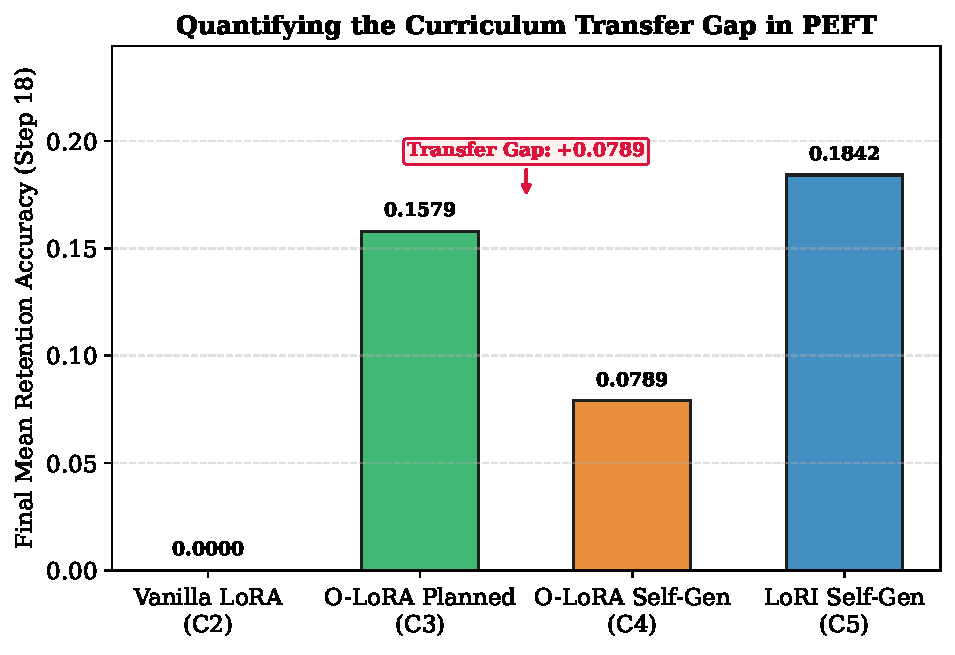
\includegraphics[width=0.48\textwidth]{figures/fig3_transfer_gap.pdf}
\caption{Quantifying the Curriculum Transfer Gap between human-planned (C3) and self-generated (C4) curricula, alongside LoRI (C5) state-of-the-art performance.}
\label{fig:transfer_gap}
\end{figure}

\begin{figure}[htbp]
\centering
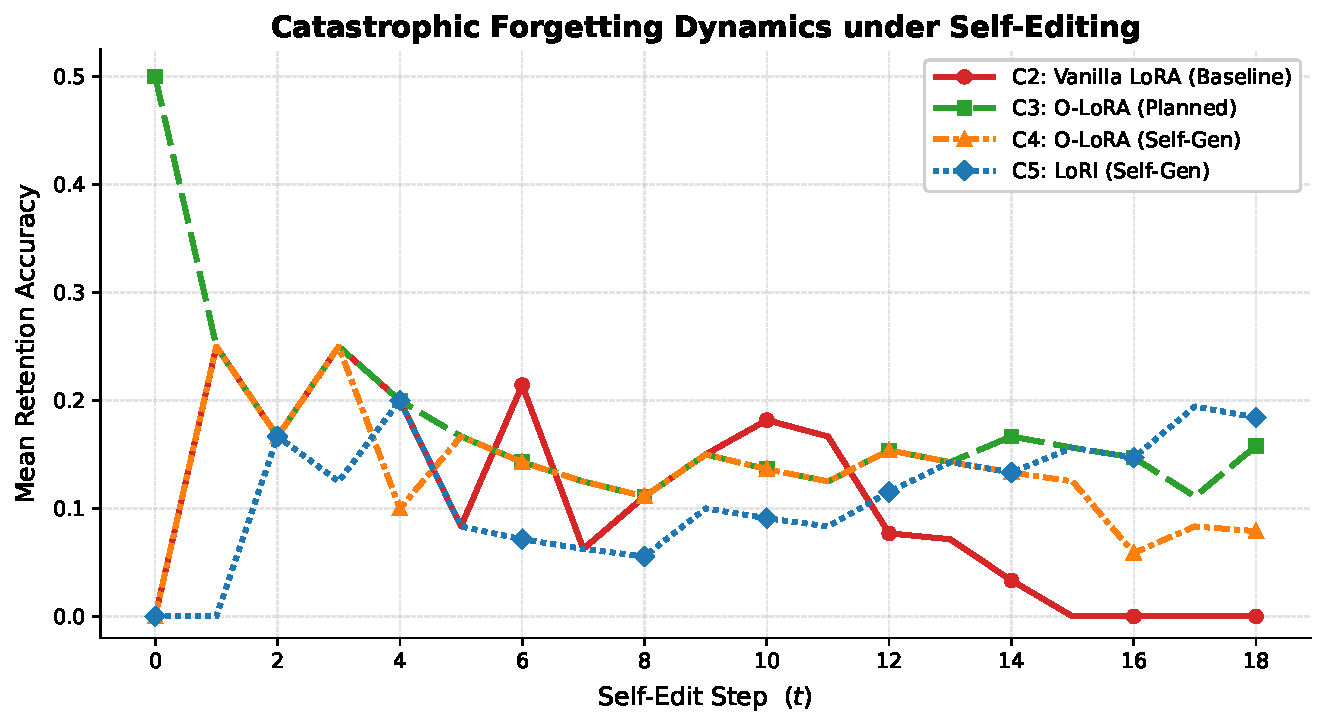
\includegraphics[width=0.48\textwidth]{figures/fig2_forgetting_curves.pdf}
\caption{Mean accuracy trajectories across self-edit sequence steps showing catastrophic collapse in C2 vs retention in C3, C4, and C5.}
\label{fig:forgetting_curves}
\end{figure}

\section{Discussion: The Curriculum Transfer Gap}
As shown in Fig.~\ref{fig:transfer_gap}, O-LoRA under a human-planned curriculum (C3) retains 15.79\% accuracy, but suffers a 7.90\% drop to 7.89\% under self-generated ordering (C4). Qualitative analysis of selection logs reveals that LLM self-selection exhibits \textit{semantic topic clustering} (e.g., selecting 3 consecutive Nobel Science facts, followed by 3 Olympic athletics facts). This burstiness leads to localized subspace crowding, where soft orthogonality loss cannot fully disentangle updates. LoRI (C5) overcomes this by freezing $A$ and sparse-masking $B$, preventing parameter drift regardless of curriculum burstiness.

\section{Conclusion}
This study provides the first formalization and empirical measurement of the Curriculum Transfer Gap in autonomous self-editing language models. Our findings demonstrate that sparse parameter projections (LoRI) outperform soft orthogonality penalties when LLMs direct their own learning paths.

\end{document}
